Given the poor results using standard feature extraction techniques and simple models, we see a few issues to tackle:

\begin{enumerate}

    \item Feature learning on the graph can not just be averaging of individual node features. A soccer team should be classified by the movement from specified nodes to other nodes. Simple features thus don't work. 


    \item The nodes within a soccer team are different from the nodes of other teams. Therefore node2vec does not generalize across teams, requiring a different feature extraction method when using random walks. 


    \item Simple models such as linear regression are not enough. Given the high complexity of networks and the relationship with game results, a more complex model such as neural networks is needed. 

\end{enumerate}

Thus we turn to a new method. Using related work on GCNs [2,6] as inspiration, we created a GCN model that iterates a ``sliding window'' across different paths within a network. 

\subsection{Construction of GCN Data}

We constructed numerous types of data to train on a GCN. Our initial idea was to measure the top-3 hops. That is, we create a vector composing the assigned node, the top 3 nodes that first node links to (in terms of passing rate), then the 9 nodes connected to those top 3 nodes. The resulting vector is of length 13 and can contain information regarding the node itself. We decided to use shot rate, loss rate, gain rate, and average pass rate to categorize the nodes. We then repeated this function for all nodes within the graph, giving us a 17x13x4 matrix for each datapoint. However, this construction had issues. 

One issue is that we are only considering top-3 hops for every graph. In reality, there may be important information in longer path lengths. Additionally, top-3 hops has the potential to only see a subset of nodes within the graph. Lastly taking a vector for each start node does not generalize well across different graphs given different number of players/player types. Simple running of the data on a simple CNN resulted in poor accuracies and losses. We therefore decided to think of a new construction that: 

\begin{enumerate}
    \item Considers all the nodes in some function when creating vectors.

    \item Generalizes better across different teams/graphs. 
\end{enumerate}

\subsection{Novel approach applying random walks and GCNs}
Our final data construction took inspiration from node2vec's random walk procedure, and Gibbs sampling [8]. Like node2vec, we simulate a random walk throughout the network but start at the ``Gain'' state. This is essentially the path of the ball during some possession.  We then assemble the data for each node along this random walk and add it to the datapoint. We repeat this for 100 steps and 100 trials, giving us a 100x100x4 matrix (similar to Gibb's sampling approaches). We can then use this 100x100x4 matrix as a representation of a graph. Given the randomness of the path sampling, this method should generalize well across epochs of training. Additionally, starting at the ``Gain'' state makes each graph consistent. Consistent sizing (100x100) also simplifies the implementation of the GCN. 


\begin{figure}[h]
  \centering
  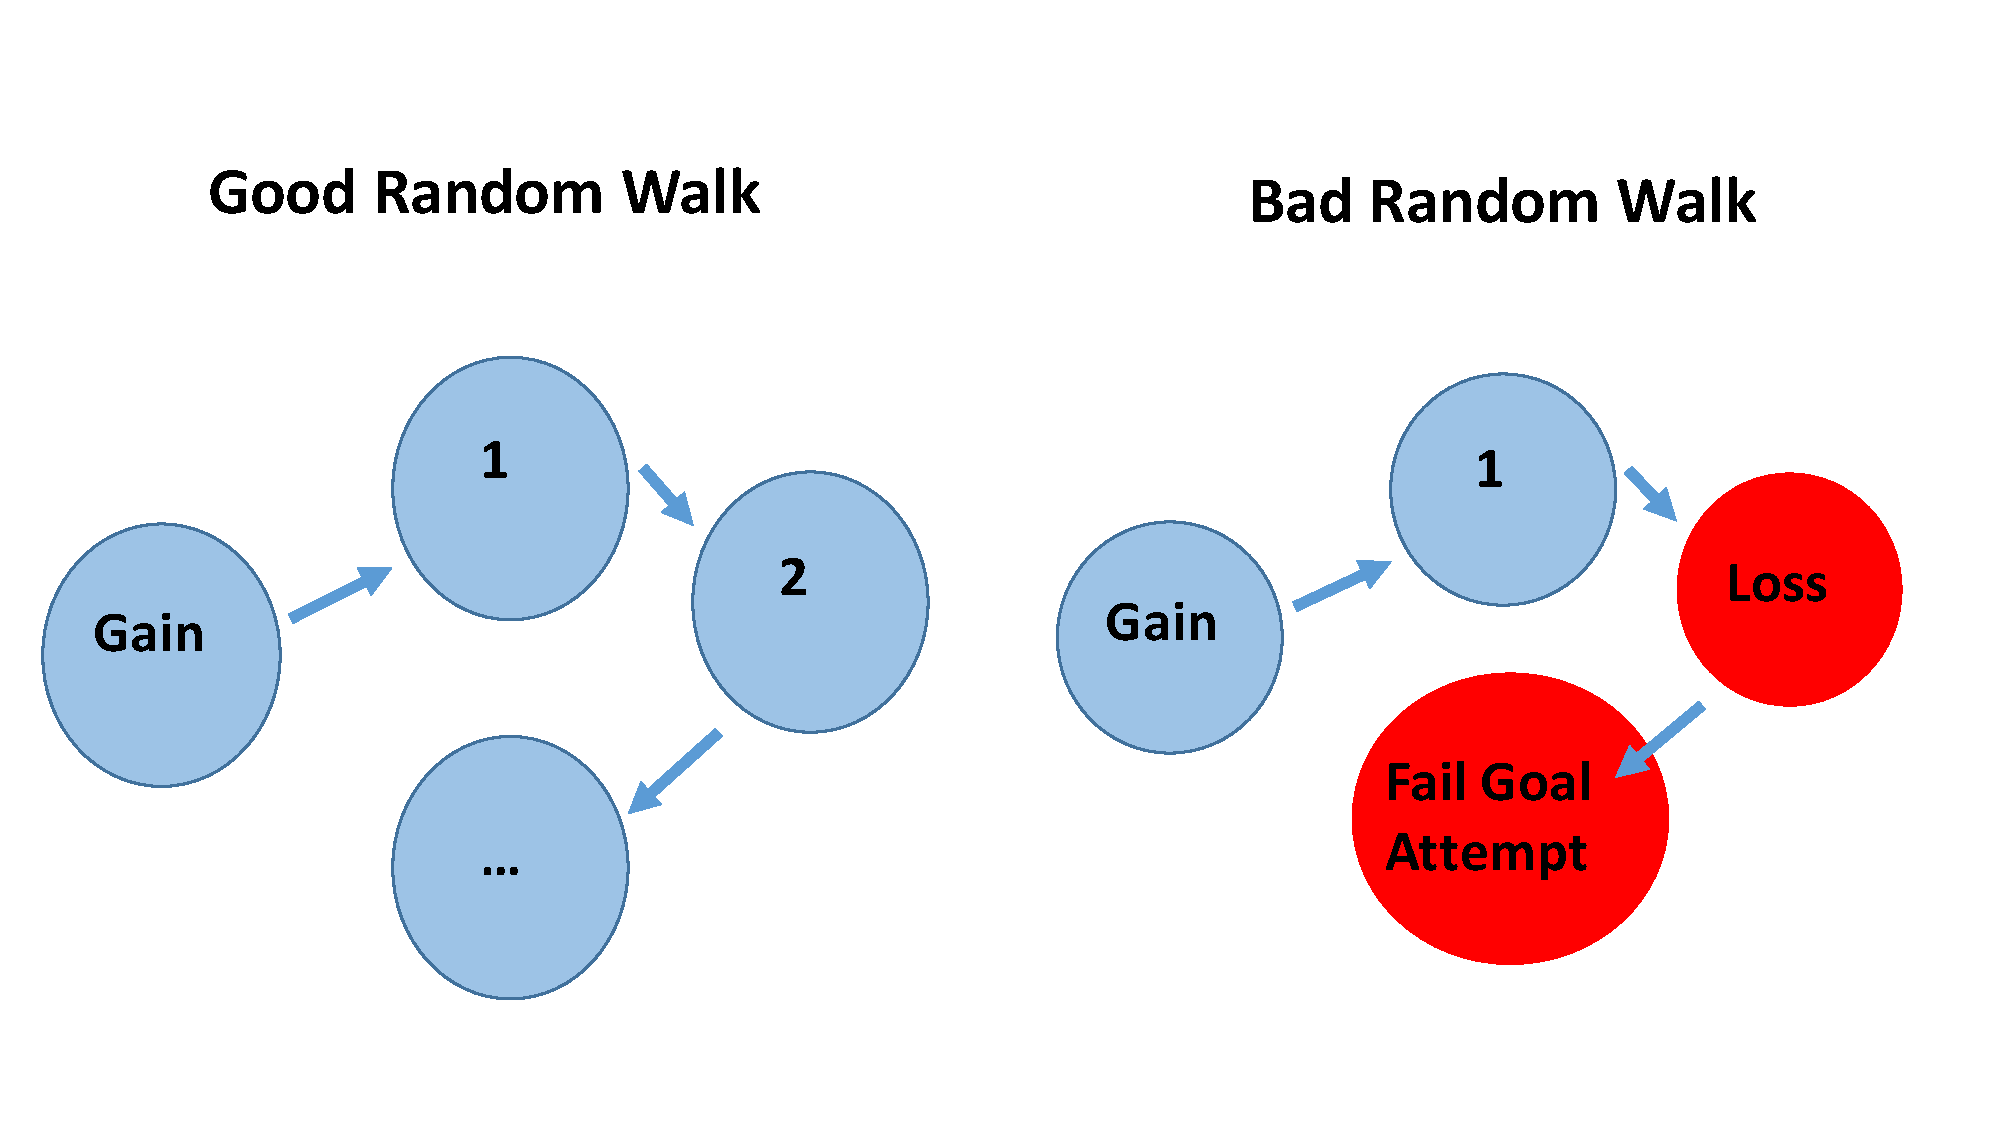
\includegraphics[width=0.45\textwidth]{plots/graph_CNN_intuition.pdf}
  \caption{We designed a \textit{novel} application of random-walks to GCNs that attempts to distinguish ``good paths'' where a team stays in possession (left) from ``bad paths'' where it quickly turns over the ball or fails to score within a long random walk (right). We use domain-specific insight to always start from ``Gain'' nodes where the team just got the ball and had the best chance of continuing its possession.}
  \label{fig:intuition}
\end{figure}

Given our data construction, we now need a GCN implementation that makes sense. We use the generic structure in CNNs: a number of convolutional layers with pooling, then fully connected layers. For our response we use win, loss, or draw. Given the random path data construction, we are trying to learn how different types of n-hop paths contribute to game results. We therefore use a non-traditional sliding window of (1,n) to learn this. This sliding window does not work on multiple paths at the same time, as we want parameter sharing across individual paths in each datapoint. The aggregation comes in the pooling layers where both average pooling and max pooling were tested. Our model architecture is shown in Figure \ref{fig:GCN_architecture}.




%\begin{enumerate}
%    \item Convolutional Layer with 20 filters and (1,10) size sliding window
%    \item RELU transform
%    \item Average pooling of size 4
%    \item Convolutional Layer with 15 filters and (1,5) size sliding window
%    \item RELU transform
%    \item Average pooling of size 2
%    \item Convolutional Layer with 10 filters and (1,3) size sliding window
%    \item RELU transform
%    \item Fully Connected Layer
%    \item RELU transform
%    \item Fully Connected Layer
%    \item RELU transform
%    \item Fully Connected Layer
%    \item Softmax Layer
%\end{enumerate}

\begin{figure}[h!]
  \centering
\begin{tabular}{l |}
    \rowcolor{gray!20}
    Custom GCN Architecture \\
    \rowcolor{blue!20}
    \pbox{20cm}{Conv. Layer with 20 filters and \\ (1,10) size sliding window} \\
    \rowcolor{green!20}
    RELU transform \\
    \rowcolor{blue!20}
    Average pooling of size 4 \\
    \rowcolor{green!20}
    \pbox{20cm}{Conv. Layer with 15 filters and \\ (1,5) size sliding window} \\
    \rowcolor{blue!20}
    RELU transform \\
    \rowcolor{green!20}
    Average pooling of size 2 \\
    \rowcolor{blue!20}
    \pbox{20cm}{Conv. Layer with 10 filters and \\ (1,3) size sliding window} \\
    %Conv. Layer with 10 filters and (1,3) size sliding window \\
    \rowcolor{green!20}
    RELU transform \\
    \rowcolor{blue!20}
    Fully Connected Layer \\
    \rowcolor{green!20}
    RELU transform \\
    \rowcolor{blue!20}
    Fully Connected Layer \\
    \rowcolor{green!20}
    RELU transform \\
    \rowcolor{blue!20}
    Fully Connected Layer \\
    \rowcolor{green!20}
    Softmax Layer \\
\end{tabular}
\caption{We implemented a custom GCN architecture to predict game outcome from learned embeddings.}
  \label{fig:GCN_architecture}
\end{figure}

\subsection{GCN Results on Random Path Data:}

The GCN was trained using cross entropy loss, stochastic gradient descent with learning rate 0.02 and momentum 0.8, and 100 epochs with batch size 60. Given these parameters, the training accuracy started at 30\% and slowly moved up to 66\% before dropping back down. This signals potential problems with the optimizer, and a decreasing learning rate should be adopted. On the test set this GCN achieved 62\% accuracy. 

The small difference in training and test accuracy can be explained by the randomness in the data construction. Given the random sampling, the model ends up reading less noise, as each epoch generates more data from the random path sampling. In the end, there is some significant features within the paths that contribute to wins, losses, and draws. Our model achieved better accuracy on losses and wins than draws. Additionally, our model did not assume the differences in wins, losses, or draws to be ordered. 

Our 62\% test accuracy is significantly better than the top accuracy of all other models tested (48\%). This increase can be attributed to a number of changes, including the path sampling for generalization, and the use of a more complex model to read complex signals. Ultimately, we find that there is information in the constructed network that contributes to end of game results. Specifically, there are sub-paths within random walks which signal that a team is performing well or not well given gain, loss, shot, and average pass rates of players. 



